\chapter{Results}
\section{Vendor Clustering}
Agglomerative Clustering\cite{ward1963hierarchical}, K-means\cite{macqueen1967some}, DBSCAN, and a Genetic Algorithm-enhanced DBSCAN (GA-DBSCAN) were evaluated to group orders based on geographic locations. Agglomerative Clustering employs a hierarchical merging approach, K-means minimizes intra-cluster variance by partitioning the data into pre-specified clusters, and DBSCAN utilizes a density-based criterion, automatically identifying outliers and clusters of arbitrary shapes without the need to predefine the number of clusters. GA-DBSCAN improves upon standard DBSCAN by using a Genetic Algorithm (GA) to dynamically optimize DBSCAN’s parameters: \(\varepsilon\) (the neighborhood radius) and \(\text{min\_samples}\) (the minimum points required to define a cluster).

Synthetic datasets were generated to realistically simulate order distributions, with locations uniformly randomized between latitudes 8° to 18° and longitudes 72° to 82°, representing diverse geographical conditions. Each synthetic order was assigned a random quantity between 50\% and 150\% of the minimum order quantity (MOQ). For the experiments, the MOQ was set to 100 units, and a buffer percentage of 20\% was adopted, resulting in an acceptable cluster quantity range from 100 to 120 units. Clustering performance was assessed on datasets comprising 25, 50, 100, 150, 200, 300, and 350 orders. Evaluation metrics included execution time, number of valid clusters (those meeting MOQ constraints), leftover orders (orders not aggregated due to either quantity constraints or geographic isolation), and silhouette scores a measure of clustering quality ranging from -1 (poor) to +1 (excellent), calculated based on intra cluster compactness and inter cluster separation.

\begin{table}[htbp]
    \centering
    \setlength{\tabcolsep}{3pt}
    \caption{Comparative Analysis of Clustering Algorithms}
    \label{tab:perf-vc}
    \begin{tabular}{lccccc}
        \toprule
        \textbf{Algorithm} & \textbf{Orders} & \textbf{Time (s)} & \textbf{Clusters} & \textbf{Outliers} & \textbf{Silh. Score} \\
        \midrule
        \multirow{7}{*}{DBSCAN}
                           & 25              & 0.002             & 7                 & 16                & 0.350                \\
                           & 50              & 0.002             & 13                & 32                & 0.330                \\
                           & 100             & 0.003             & 28                & 68                & 0.392                \\
                           & 150             & 0.004             & 39                & 99                & 0.380                \\
                           & 200             & 0.005             & 63                & 118               & 0.375                \\
                           & 300             & 0.009             & 85                & 187               & 0.361                \\
                           & 350             & 0.010             & 98                & 219               & 0.355                \\
        \midrule
        \multirow{7}{*}{GA-DBSCAN}
                           & 25              & 0.020             & 0                 & 25                & N/A                  \\
                           & 50              & 0.025             & 0                 & 50                & N/A                  \\
                           & 100             & 0.025             & 11                & 89                & 0.735                \\
                           & 150             & 0.030             & 12                & 138               & 0.780                \\
                           & 200             & 0.036             & 39                & 156               & 0.726                \\
                           & 300             & 0.048             & 35                & 262               & 0.715                \\
                           & 350             & 0.055             & 45                & 301               & 0.629                \\
        \midrule
        \multirow{7}{*}{K-means}
                           & 25              & 0.030             & 6                 & 18                & 0.358                \\
                           & 50              & 0.004             & 12                & 34                & 0.324                \\
                           & 100             & 0.004             & 26                & 72                & 0.392                \\
                           & 150             & 0.005             & 37                & 103               & 0.390                \\
                           & 200             & 0.032             & 61                & 122               & 0.385                \\
                           & 300             & 0.007             & 84                & 189               & 0.363                \\
                           & 350             & 0.008             & 94                & 227               & 0.350                \\
        \midrule
        \multirow{7}{*}{Agglomerative}
                           & 25              & 0.002             & 6                 & 18                & 0.341                \\
                           & 50              & 0.002             & 12                & 34                & 0.337                \\
                           & 100             & 0.002             & 27                & 70                & 0.393                \\
                           & 150             & 0.004             & 38                & 101               & 0.358                \\
                           & 200             & 0.005             & 61                & 122               & 0.359                \\
                           & 300             & 0.007             & 84                & 189               & 0.359                \\
                           & 350             & 0.009             & 95                & 225               & 0.349                \\
        \bottomrule
    \end{tabular}
\end{table}

As shown in Table~\ref{tab:perf-vc}, GA-DBSCAN consistently provided the highest clustering quality, evidenced by superior silhouette scores (0.629–0.780) in datasets of 100 orders and above. However, GA-DBSCAN yielded no valid clusters for smaller datasets (25 and 50 orders), primarily because the genetic algorithm optimization was not beneficial for datasets with limited points. In these smaller scenarios, DBSCAN, K-means, and Agglomerative clustering achieved more effective results, with DBSCAN offering the fastest performance and minimal computational overhead.

For larger datasets (100 orders or more), GA-DBSCAN demonstrated significant advantages due to its adaptive tuning of \(\varepsilon\) and \(\text{min\_samples}\), optimizing clustering parameters dynamically for each dataset. Conversely, K-means and Agglomerative clustering consistently produced higher numbers of clusters and leftover orders due to their static parameterization, often resulting in over-segmentation or the inability to flexibly handle noise points. Additionally, standard DBSCAN, although computationally efficient, exhibited limitations due to its static parameter selection, leading to less coherent clusters and increased leftover orders as dataset sizes grew.

Leftover orders represent those that could not be aggregated due to either insufficient cumulative quantity to meet MOQ constraints or geographic isolation making clustering impractical. The silhouette score quantifies clustering quality, computed as the mean intra-cluster distance compared to the mean nearest-cluster distance, thus indicating how compact and well-separated the clusters are.

This evaluation clearly supports adopting a hybrid clustering strategy. Specifically, DBSCAN is computationally efficient and effective for smaller datasets (fewer than 100 orders), where dataset complexity does not justify extensive parameter tuning. For larger and more complex order distributions (100 or more orders), GA-DBSCAN is strongly recommended, given its superior clustering accuracy and effectiveness in handling noise, ensuring clusters align optimally with real-world operational constraints.

\section{Route Optimization}
\begin{table}[htbp]
    \centering
    \small
    \caption{Algorithm Performance Comparison for Route Optimization}
    \label{tab:perf-ro}
    \begin{tabular}{lcrrrr}
        \toprule
        \textbf{Algorithm} & \textbf{Vendors} & \textbf{Dist. (km)} & \textbf{Cost (Rs.)} & \textbf{Time (s)} \\
        \midrule
        \multirow{3}{*}{EAACO}
                           & 20               & 5197.54             & 29811.51            & 23.26             \\
                           & 50               & 8333.63             & 47618.80            & 50.43             \\
                           & 100              & 9648.29             & 54444.64            & 148.69            \\
        \midrule
        \multirow{3}{*}{EAGA}
                           & 20               & 4703.90             & 22320.78            & 20.53             \\
                           & 50               & 6993.30             & 33770.55            & 60.75             \\
                           & 100              & 8581.06             & 40956.56            & 142.21            \\
        \bottomrule
    \end{tabular}
\end{table}
As shown in Table~\ref{tab:perf-ro}, the EAGA outperformed EAACO\cite{dorigo1997ant}, which was modified to incorporate the same environmental constraints as EAGA, in both travel distance and execution time. For 20 vendors, EAGA generated routes covering 4703.90 km in 20.53 seconds, while EAACO required 23.26 seconds to produce routes spanning 5197.54 km. With 50 vendors, EAGA optimized the route to 6993.30 km in 60.75 seconds, whereas EAACO produced routes covering 8333.63 km in 50.43 seconds. For 100 vendors, EAGA achieved routes of 8581.06 km in 142.21 seconds, while EAACO took 148.69 seconds to generate routes of 9648.29 km. EAGA performed better due to its faster convergence and effective balance between exploration and exploitation, whereas EAACO required more iterations to refine paths, leading to higher travel distances and execution times despite using identical environmental data inputs.


\section{Demand Forecasting}
\par The NeuralProphet model was evaluated using the Store Item Demand Forecasting Challenge dataset, which provides historical daily sales data for multiple store-item combinations. For our analysis, we specifically focused on item 1 from the dataset to demonstrate the model's performance on a representative product time series. Performance was assessed using standard error metrics to evaluate forecasting accuracy across different learning rate and training epoch.

\begin{figure}[htbp]
    \centering
    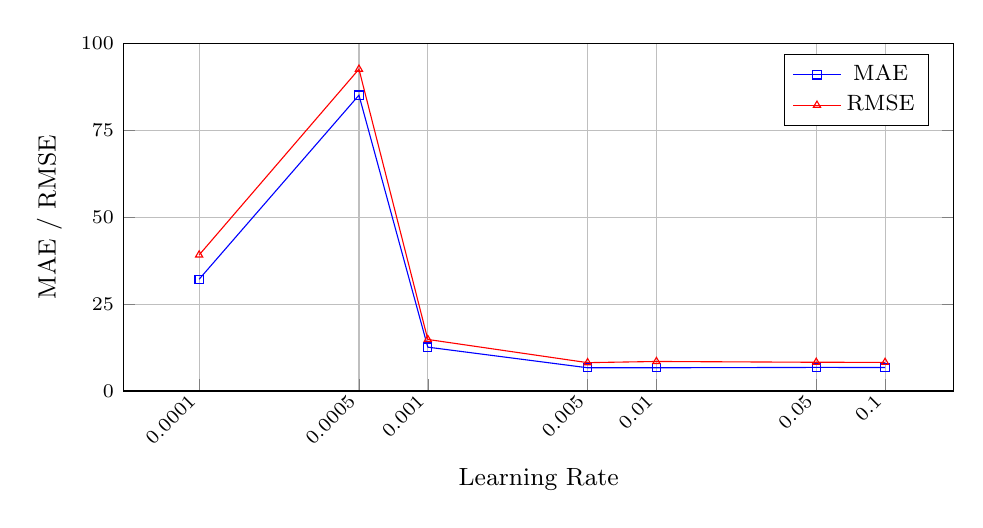
\begin{tikzpicture}
        \begin{axis}[
                width=1\columnwidth, % Control width explicitly
                height=6cm,           % Control height
                xmode=log,            % Log scale for x-axis
                xlabel={Learning Rate},
                ylabel={MAE / RMSE},
                legend pos=north east,
                grid=major,
                xmax=0.2,
                ymin=0, ymax=100,
                xtick={0.0001, 0.0005,0.001, 0.005,0.01, 0.05,0.1},  % Fewer ticks
                xticklabels={0.0001, 0.0005,0.001, 0.005,0.01, 0.05,0.1}, % Scientific notation
                xtick pos=left,
                x tick label style={rotate=45, anchor=east},
                ytick={0, 25, 50, 75, 100},
                ymajorgrids=true,
                xmajorgrids=true,
                tick label style={font=\scriptsize}, % Even smaller tick labels
                label style={font=\small},
                legend style={font=\footnotesize}, % Smaller legend
            ]

            % Plot MAE (same data, just visual changes)
            \addplot[color=blue, mark=square, mark size=1.5pt]
            coordinates {
                    (0.0001, 32.14) (0.0005, 85.04) (0.001, 12.62)
                    (0.005, 6.69) (0.01, 6.69) (0.05, 6.79) (0.1, 6.77)
                };
            \addlegendentry{MAE}

            % Plot RMSE (same data, just visual changes)
            \addplot[color=red, mark=triangle, mark size=1.5pt]
            coordinates {
                    (0.0001, 39.12) (0.0005, 92.52) (0.001, 14.83)
                    (0.005, 8.16) (0.01, 8.50) (0.05, 8.27) (0.1, 8.25)
                };
            \addlegendentry{RMSE}
        \end{axis}
    \end{tikzpicture}
    \caption{Effect of learning rate on MAE and RMSE for NeuralProphet model}
    \label{fig:np_learning_rate}
\end{figure}

\par Fig.~\ref{fig:np_learning_rate} illustrates the impact of learning rate on model accuracy. Both error metrics exhibit a characteristic U-shaped pattern, with optimal performance achieved at learning rates between 0.005 and 0.01. At extremely low rates (0.0001), the model converges slowly, resulting in higher errors (MAE=32.14, RMSE=39.12). Interestingly, at 0.0005, performance significantly deteriorates (MAE=85.04, RMSE=92.52), likely due to the optimizer becoming trapped in a poor local minimum. As learning rates increase beyond 0.01, error metrics stabilize, indicating the model's robustness across a range of higher learning rates. The optimal learning rate of 0.005 achieves the lowest MAE (6.69) and RMSE (8.16).

\begin{figure}[htbp]
    \centering
    \begin{tikzpicture}
        \begin{axis}[
                width=1\columnwidth, % Control width explicitly
                height=6cm,
                xlabel={Epochs},
                ylabel={MAE / RMSE},
                legend pos=north east,
                grid=major,
                xmin=-25, xmax=525,
                ymin=0, ymax=300,
                xtick={0,100,200,300,400,500},
                xticklabels={0,100,200,300,400,500},
                ymajorgrids=true,
                xmajorgrids=true,
            ]

            % Load MAE data from file
            \addplot[
                color=blue,
                mark=none, % No markers for large datasets
            ]
            table[x=Epoch, y=MAE, col sep=comma] {./Figures/mae_rmse_metrics.csv};
            \addlegendentry{MAE}

            % Load RMSE data from file
            \addplot[
                color=red,
                mark=none, % No markers for large datasets
            ]
            table[x=Epoch, y=RMSE, col sep=comma] {./Figures/mae_rmse_metrics.csv};
            \addlegendentry{RMSE}
        \end{axis}
    \end{tikzpicture}
    \caption{Effect of Epochs on MAE and RMSE for NeuralProphet model}
    \label{fig:np_mae_rmse}
\end{figure}


\section{Cost Comparison Analysis}
To evaluate the effectiveness of the proposed collaborative ordering and shared delivery model, we analyzed route optimization performance across 50 vendors, comparing traditional individual delivery routes against our collaborative approach. In the 50-vendor scenario presented in Table~\ref{tab:cost-comparison}, our system processed five staggered orders of varying sizes, analyzing both traditional and collaborative routing methods. The traditional approach required five separate delivery routes, often with significant overlap. In contrast, our collaborative model consolidated these into a single optimized route, yielding substantial savings in distance, cost, and fuel consumption.
\begin{itemize}
    \item {Scenario:} 50 vendors requiring deliveries from a central supplier
    \item {Traditional approach:} Individual routes planned for each vendor or small group
    \item {Collaborative approach:} Single optimized route serving all vendors
    \item {Distance analyzed:} Regional delivery network covering approximately 7,000 km
\end{itemize}

\begin{table}[htbp]
    \centering
    \caption{Cost Comparison: Traditional vs. Collaborative Route Optimization}
    \label{tab:cost-comparison}
    \begin{tabular}{lrrr}
        \toprule
        \textbf{Metric}  & \textbf{Trad. Approach} & \textbf{Collab. Approach} & \textbf{Savings} \\
        \midrule
        Distance (km)    & 35,606                  & 6,993                     & 28,613 (80.4\%)  \\
        Route Cost (Rs.) & 36,929                  & 7,255                     & 29,675 (80.4\%)  \\
        Fuel (L)         & 1,811                   & 357                       & 1,454 (80.3\%)   \\
        Fuel Cost (Rs.)  & 171,135                 & 33,770                    & 137,366 (80.3\%) \\
        \bottomrule
    \end{tabular}
\end{table}


\par Fig.~\ref{fig:np_mae_rmse} demonstrates how error metrics evolve over training epochs. Both MAE and RMSE follow similar trajectories, decreasing rapidly during the initial 100 epochs, followed by gradual refinement and eventual convergence around 400 epochs. This pattern reflects the typical learning dynamics of neural network-based forecasting models—quick initial gains followed by diminishing returns as training progresses. The relatively smooth convergence curve indicates stable training dynamics without significant oscillations, suggesting appropriate hyperparameter settings.


\begin{figure}[htbp]
    \centering
    \begin{tikzpicture}
        \begin{axis}[
                width=\columnwidth,
                height=6cm,
                xlabel={Time Period},
                ylabel={Order Quantity},
                legend pos=north west,
                grid=both,
                date coordinates in=x,
                xticklabel={\year},
                xticklabel style={rotate=45, anchor=north east},
                xtick distance=365,
                date ZERO=2023-01-01,  % Reference start date
                ymajorgrids=true,
                xmajorgrids=true,
                legend style={font=\footnotesize},
                legend cell align={left},
            ]

            % Actual data from training dataset
            \addplot[
                blue,
                thick,
                smooth
            ]
            table[
                    x=ds,
                    y=y,
                    col sep=comma
                ] {Figures/np_train_data.csv};
            \addlegendentry{Orders}

            % Forecasted data
            \addplot[
                red,
                thick,
                smooth
            ]
            table[
                    x=ds,
                    y=yhat1,
                    col sep=comma
                ] {Figures/forecast.csv};
            \addlegendentry{Forecast}
        \end{axis}
    \end{tikzpicture}
    \caption{NeuralProphet Demand Forecasting}
    \label{fig:forecast}
\end{figure}
\begin{figure}[htbp]
    \centering
    \begin{tikzpicture}
        \begin{axis}[
                width=\columnwidth,
                height=6cm,
                xlabel={Year},
                ylabel={Order Quantity},
                legend pos=north west,
                grid=both,
                date coordinates in=x,
                xtick={2018-01-01, 2019-01-01, 2020-01-01, 2021-01-01, 2022-01-01, 2023-01-01, 2024-01-01,2025-01-01},
                xticklabels={2018, 2019, 2020, 2021, 2022, 2023, 2024,2025},
                xticklabel style={rotate=45, anchor=north east},
                date ZERO=2018-01-01,
                ymajorgrids=true,
                xmajorgrids=true,
                legend style={font=\footnotesize},
                legend cell align={left},
            ]

            % Actual data from training dataset
            \addplot[
                blue,
                thick,
            ]
            table[
                    x=ds,
                    y=trend,
                    col sep=comma
                ] {Figures/forecast_whole.csv};
            \addplot[
                red,
                thick,
            ]
            table[
                    x=ds,
                    y=trend,
                    col sep=comma
                ] {Figures/forecast.csv};
        \end{axis}
    \end{tikzpicture}
    \caption{NeuralProphet Long-term Trend Analysis}
    \label{fig:trend}
\end{figure}
\begin{figure}[htbp]
    \centering
    \begin{tikzpicture}
        \begin{axis}[
                width=\columnwidth,
                height=6cm,
                xlabel={Day of Week},
                ylabel={Seasonal Effect},
                legend pos=north west,
                grid=both,
                ytick={-30,-20,-10,0,10,20,30},              % Specify exact tick positions
                yticklabels={-30,-20,-10,0,10,20,30},
                xtick={0,1,2,3,4,5,6,7},
                xticklabels={Sunday,Monday,Tuesday,Wednesday,Thursday,Friday,Saturday,Sunday},
                xticklabel style={rotate=45, anchor=north east},
                ymajorgrids=true,
                xmajorgrids=true,
                legend style={font=\footnotesize},
                legend cell align={left},
            ]

            % Actual data from training dataset - only first 7 entries with smooth curve
            \addplot[
                blue,
                thick,
                smooth,
                tension=0.4, % Add some tension for a smoother curve
            ]
            table[
                    x expr=\coordindex, % Use index as x-coordinate instead of date
                    y=season_weekly,
                    col sep=comma,
                    restrict expr to domain={\coordindex}{0:7}
                ] {Figures/forecast.csv};
        \end{axis}
    \end{tikzpicture}
    \caption{NeuralProphet Weekly Seasonality Analysis}
    \label{fig:weekly-seasonality}
\end{figure}
\begin{figure}[H]
    \centering
    \begin{tikzpicture}
        \begin{axis}[
                width=\columnwidth,
                height=6cm,
                xlabel={Month},
                ylabel={Seasonal Effect},
                legend pos=north west,
                grid=both,
                date coordinates in=x,
                ytick={-60,-40,-20,0,20,40,60},              % Specify exact tick positions
                yticklabels={-60,-40,-20,0,20,40,60},
                xticklabel={\month}, % Show just month number
                xtick distance=91.5,  % Approximately monthly ticks
                date ZERO=2023-01-01,
                xtick={2023-01-01,2023-03-01,2023-05-01,2023-07-01,2023-09-01,2023-11-01,2024-01-01}, % Explicit tick positions
                xticklabels={Jan,Mar,May,Jul,Sep,Nov,Jan}, % Month labels
                xticklabel style={rotate=45, anchor=north east},
                ymajorgrids=true,
                xmajorgrids=true,
                legend style={font=\footnotesize},
                legend cell align={left},
            ]

            % Actual data from training dataset
            \addplot[
                blue,
                thick,
                smooth,
                tension=0.4
            ]
            table[
                    x=ds,
                    y=season_yearly,
                    col sep=comma
                ] {Figures/forecast.csv};
        \end{axis}
    \end{tikzpicture}
    \caption{NeuralProphet Yearly Seasonality Analysis}
    \label{fig:yearly-seasonality}
\end{figure}
\par Fig.~\ref{fig:forecast} illustrates NeuralProphet's ability to predict future order quantities based on historical data, providing vendors with reliable projections for inventory planning. Supporting this predictive capability, Fig.~\ref{fig:trend} reveals the underlying long-term growth trajectory that informs strategic business decisions and expansion planning. Further enhancing these insights, Fig.~\ref{fig:weekly-seasonality} and Fig.~\ref{fig:yearly-seasonality} demonstrate how our model accurately captures both weekly variations and annual seasonal patterns in vendor ordering behavior. This comprehensive forecasting capability is crucial for vendors and suppliers to anticipate demand fluctuations, optimize inventory management, and plan logistics operations efficiently throughout the year.
